\chapter{Návrh řešení virtualizace síťových funkcí}

V předchozí kapitole byly popsány technologie, které byly v této práci použity. V této kapitole bude uvedeno několik příkladů, jak lze jednoduše vytvořit VNF v prostředí OpenStack a OpenContrail pomocí heat templatů. Všechna uvedená řešení byla testována v prostředí OpenStack s OpenContrailem, které bylo pro tyto účely poskytnuto společností tcp cloud a.s.


Následující diagram znázorňuje logickou architekturu navrženého řešení dle referenční architektury zmíněné v kapitole 2.4. OpenStack spolu s OpenContrailem poskytují NFV infrastrukturu jednotlivé VNF jsou řízeny pomocí Heat.

\begin{figure}[h]
\begin{centering}
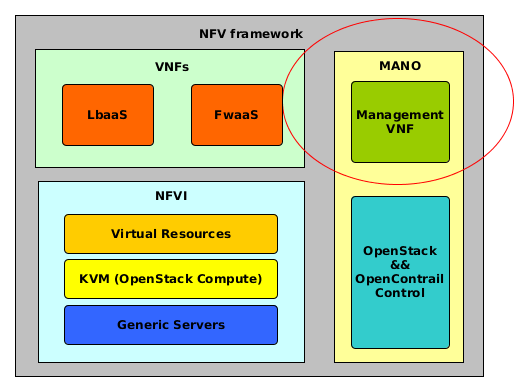
\includegraphics[scale=0.51]{images/VNF_overview}
\par\end{centering}
\caption{Architektura NFV řešení\label{fig:VNF_overview}}
\end{figure}

\section{Heat template pro LbaaS}\label{sub:interaction}

Navržený heat template pro LbaaS v sobě obsahuje následující prostředky, které se po spuštění pokusí vytvořit.

\begin{itemize}
\item pool
\item members
\item health monitoring
\item 2 web instance
\item privatni síť
\item public síť
\end{itemize}

\subsection{Testování LbaaS}\label{sub:interaction}

Pro vytvoření heat stacku s Load balancerem je nutné daný template vytvořit pomocí příkazu:

\verb!heat stack-create -f heat/templates/lbaas_template.hot -e heat/env/lbaas_env.env lbaas!

Tento příkaz vytvoří všechny již uvedené prostředky pro load balancing. Konkrétní load balancer má nakonfigurovanou virtual ip adresu (VIP) a k ní přiřazenou floating adresu, která je přístupná z externích sítí. Zároveň má tento load balancer přiřazený pool, ke kterému je přiřazena přiřazena privátní síť 10.10.10.0/24. Na obrázku č. X znázorňuje tento pool a obrázek č. X+1 jsou vidět členové (members) toho poolu.

\begin{figure}[h]
\begin{centering}
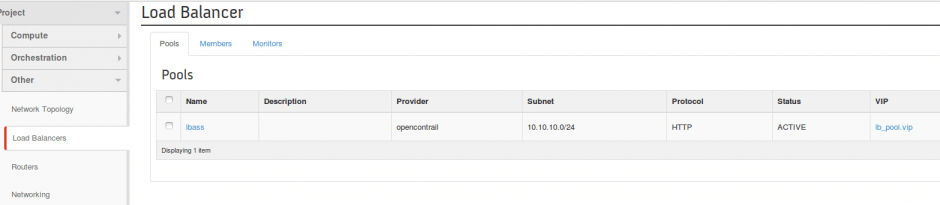
\includegraphics[scale=0.45]{images/lbaas1}
\par\end{centering}
\caption{Vytvořený pool\label{fig:lbaas1}}
\end{figure}

\begin{figure}[h]
\begin{centering}
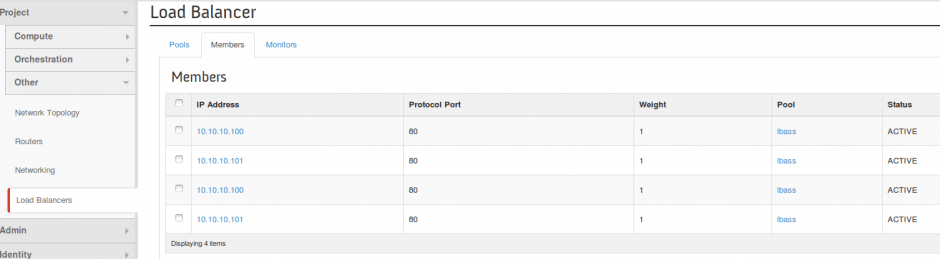
\includegraphics[scale=0.45]{images/lbaas2}
\par\end{centering}
\caption{Vytvoření members\label{fig:lbaas2}}
\end{figure}

Další zdrojem, který byl vytvořen je health monitor, který lze viděn na obrázku č. X+2. Díky němu má load balancer přehled o aktuálním stavu webových instancí. Pokud by náhodou některá z nich přestala odpovídat, v tomto případě na ping, tak by load balancer na tuto instanci přestal zasílat traffic.

\begin{figure}[h]
\begin{centering}
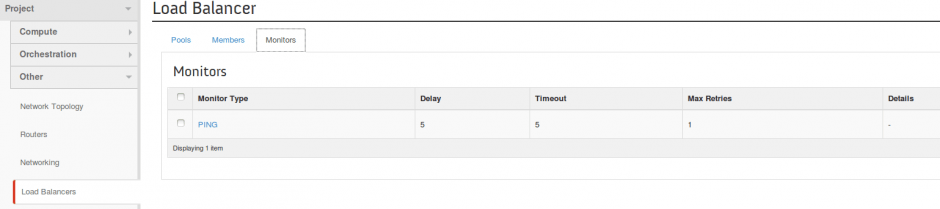
\includegraphics[scale=0.45]{images/lbaas3}
\par\end{centering}
\caption{Vytvořený health monitor\label{fig:lbaas3}}
\end{figure}

Finální síťovou topologii znázorňuje obrázek č. X+3. 


\begin{figure}[h]
\begin{centering}
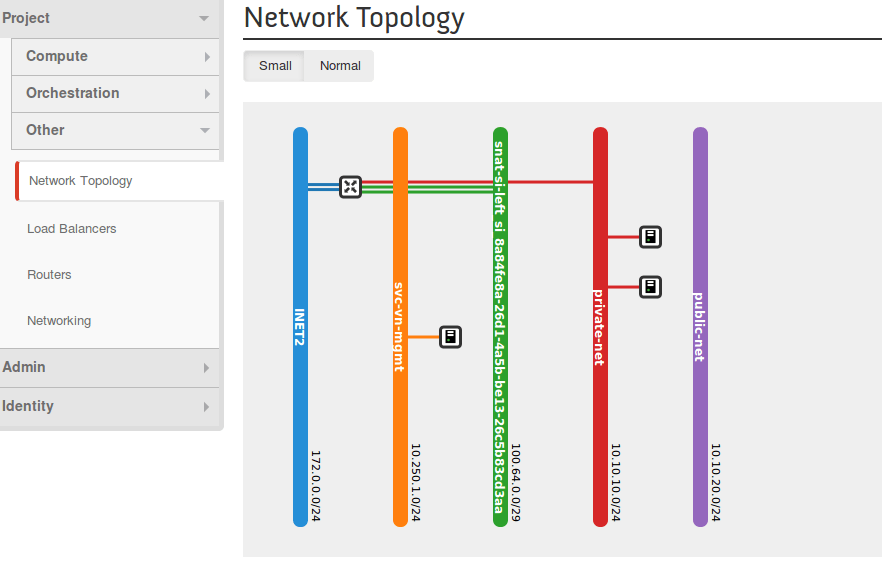
\includegraphics[scale=0.45]{images/lbaas_topologie}
\par\end{centering}
\caption{Vytvořená síťová topologie\label{fig:lbaas_topologie}}
\end{figure}

Otestování webových serverů lze provést příkazem curl, kterému dáme jako paramert ip VIP nebo floating ip load balanceru. Po několika takovýchto zadání tohoto příkazu je vidět, že oba web servery odpovídají a je probíhá mezi nimi load balancing metodou round robin.  Celý tento test je vidět na obr. č. X+4

\begin{figure}[h]
\begin{centering}
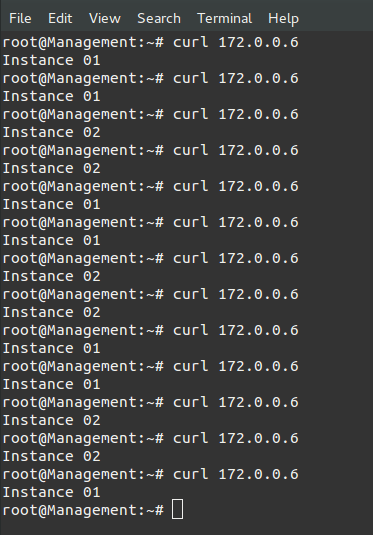
\includegraphics[scale=0.45]{images/lbaas_testing}
\par\end{centering}
\caption{Test konektivity a load balancingu\label{fig:lbaas_testing}}
\end{figure}


\section{Heat template pro FwaaS}\label{sub:interaction}

Pro FwaaS je narhnut heat template, který obsahuje:

\begin{itemize}
\item 1 firewall instanci
\item 1 testovaci instanci
\item 1 management instanci
\item management síť
\item privátní síť
\item contrail policy
\end{itemize}


\subsection{Testování FwaaS}\label{sub:interaction}

Pro vytvoření heat stacku s PFSense z templatu lze použít příkaz:

\verb!heat stack-create -f heat/templates/fwaas_mnmg_template.hot -e heat/env/fwaas_pfsense_env.env pfsense!

a pro vytvoření heat stacku s Fortigate VM jde vytvořit pomocí příkazu:

\verb!heat stack-create -f heat/templates/fwaas_mnmg_template.hot -e heat/env/fwaas_fortios_contrail.env fortios!


\begin{figure}[h]
\begin{centering}
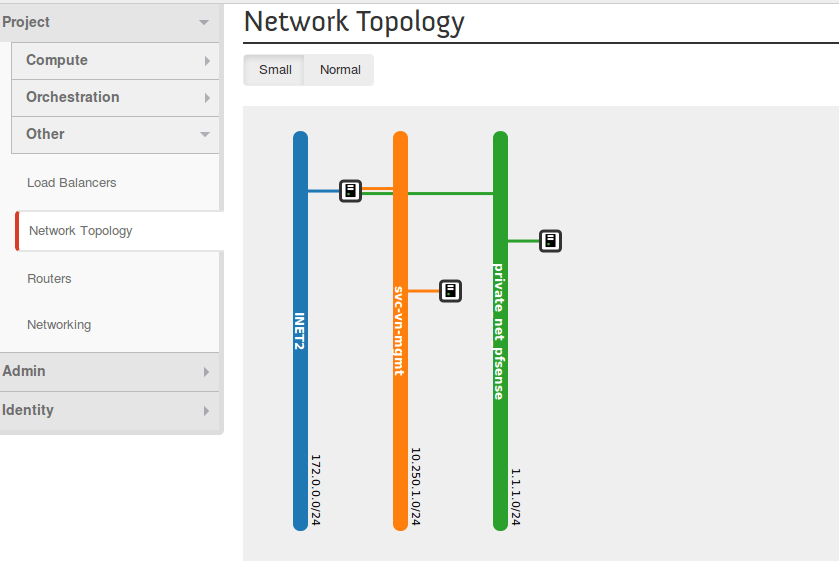
\includegraphics[scale=0.45]{images/fwaas_topologie}
\par\end{centering}
\caption{Síťová topologie\label{fig:fwaas_topologie}}
\end{figure}


By default, pfsense firewall is configured to NAT after the heat stack is started. As a result, there is no need to make any configuration for this function. Pfsense image was preconfigured with DHCP services on every interface and there is outbound policy for NAT.

After we start the heat with pfsense there is already functional service chaining. Testing instance has default gateway to contrail and contrail redirects it to pfsense.

\begin{figure}[h]
\begin{centering}
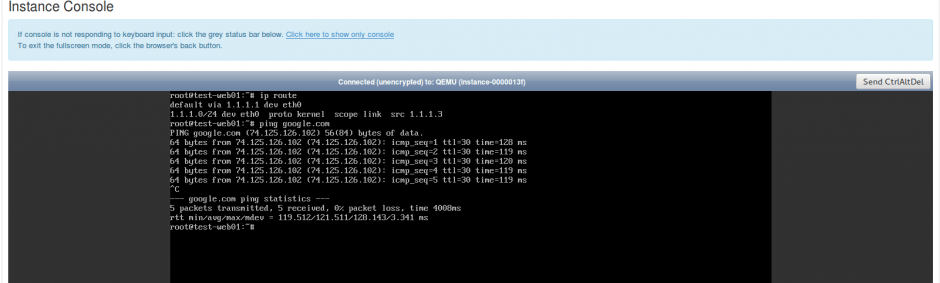
\includegraphics[scale=0.45]{images/pfsense_ping}
\par\end{centering}
\caption{Test konektivity PFSense\label{fig:pfsense_ping}}
\end{figure}

\begin{figure}[h]
\begin{centering}
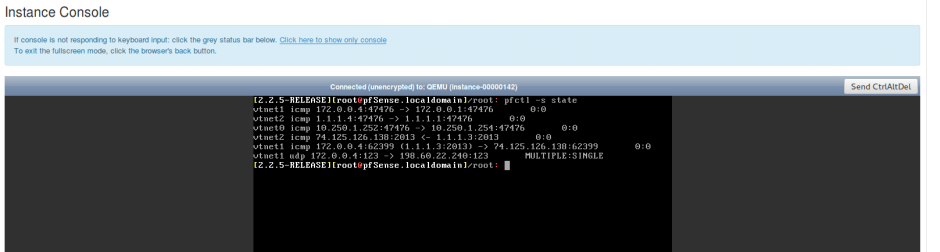
\includegraphics[scale=0.45]{images/pfsense_nat}
\par\end{centering}
\caption{Ukázka NAT session\label{fig:pfsense_nat}}
\end{figure}

There is also NAT session in pfsense. In shell run command:

\begin{figure}[h]
\begin{centering}
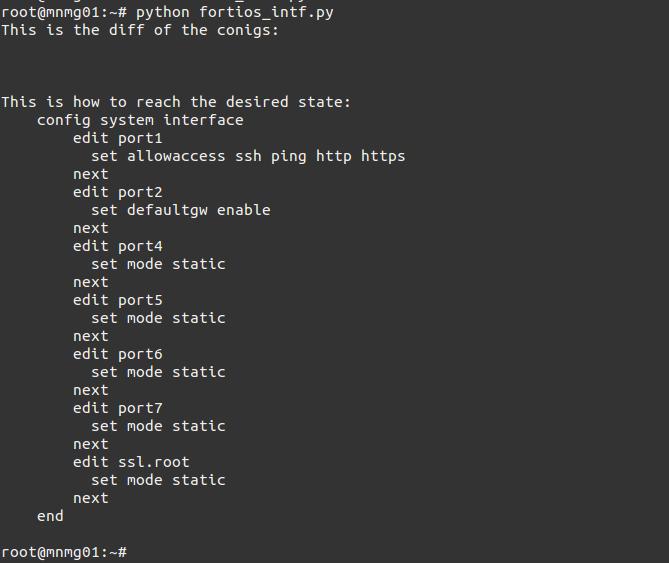
\includegraphics[scale=0.45]{images/fortigate_int}
\par\end{centering}
\caption{Fortigate VM intergace konfigurace\label{fig:fortigate_int}}
\end{figure}

\begin{figure}[h]
\begin{centering}
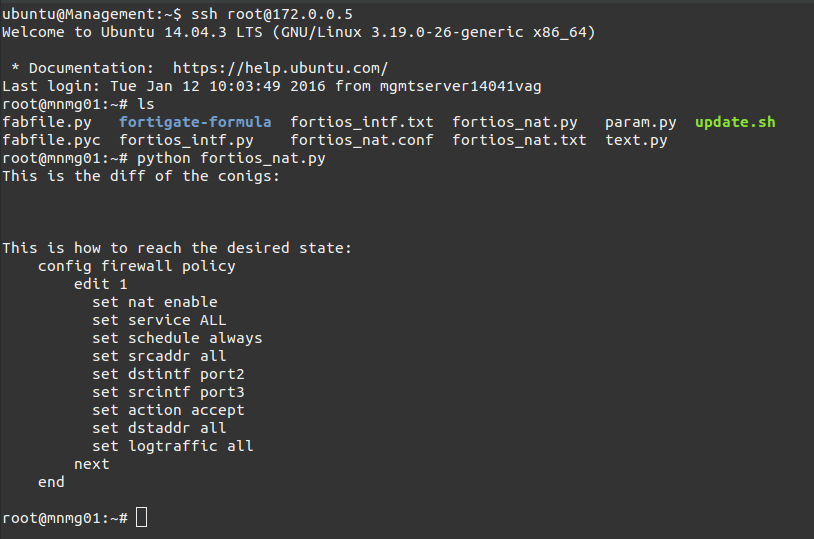
\includegraphics[scale=0.45]{images/fortigate_nat}
\par\end{centering}
\caption{Fortigate VM NAT konfigurace\label{fig:fortigate_nat}}
\end{figure}

\begin{figure}[h]
\begin{centering}
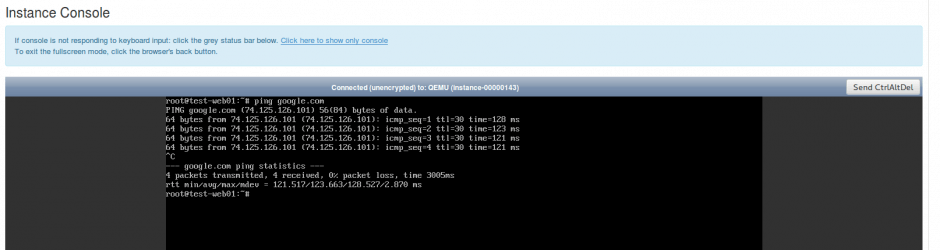
\includegraphics[scale=0.45]{images/fortigate_ping}
\par\end{centering}
\caption{Test konektivity\label{fig:fortigate_ping}}
\end{figure}
